\documentclass[12pt,unknownkeysallowed,aspectratio=169,usenames,dvipsnames]{beamer}
\usepackage{myStyle}

%%%%%%%%%%%%%%%%%%%%%%%%%%%%%%%%%%%%%%%%%%%%%%%%%%%%%%%%%%%%%%%%%%%%%%

\title[ccECPs in QMCPACK] {\large \bf Correlation Consistent ECPs and QMCPACK} 
\subtitle{QMCPACK User Meeting\\ Oak Ridge National Laboratories. Oak Ridge, TN}
\author
{ \normalsize{Cody A. Melton}\\
  \small{M.C. Bennett, A. Annaberdiyev, G. Wang, L. Shulenburger, \& L. Mitas}}
%\institute[NCSU]
%{
%    Department of Physics, North Carolina State University, Raleigh, NC \\
%    High Energy Density Physics Theory, Sandia National Laboratories, Albuquerque, NM
%}
\subject{QMC}
\date{}

\pgfdeclareimage[height=0.6cm]{argonne}{cms-figures/argonne}
\pgfdeclareimage[height=0.6cm]{berkley}{cms-figures/berkley}
\pgfdeclareimage[height=0.6cm]{sandia-brick}{cms-figures/sandia-brick}
\pgfdeclareimage[height=0.5cm]{livermore}{cms-figures/livermore}
\pgfdeclareimage[height=0.9cm]{cms}{cms-figures/cms}
\pgfdeclareimage[height=1.0cm]{doe}{cms-figures/doe}
\pgfdeclareimage[height=0.6cm]{university-logo}{cms-figures/ncsu}
\pgfdeclareimage[height=0.6cm]{ornl}{cms-figures/ornl}
\titlegraphic{
 \vspace{-20pt}
 \pgfuseimage{doe}
 \hspace{30pt}
 \pgfuseimage{cms} \\
 \vspace{8pt}
 \pgfuseimage{argonne}
 \hfill
 \pgfuseimage{berkley}
 \hfill
 \pgfuseimage{livermore}
 \hfill
 \pgfuseimage{university-logo}
 \hfill
 \pgfuseimage{ornl}
 \hfill
% \hspace{\dimexpr\paperwidth-1.75cm-5pt}
 \pgfuseimage{sandia-brick}
}


\begin{document}

\setbeamertemplate{section in toc}{\inserttocsectionnumber.~\inserttocsection}

\begin{frame}
    \titlepage
\end{frame}

\section{Introduction}
\subsection{Introduction}
\begin{frame}
    \small
    \begin{columns}
	\begin{column}
	    {0.75\textwidth}
            %{\color{darkblue}New generation of Transition Metal ECPs}\\
            For accurate calculations of functional materials (e.g. perovskites), explicitly correlated methods like QMC need to be solving the {\em correct} Hamiltonian. \\
            \bigskip 
            Effective Core Potentials (ECPs) are necessary in order to feasibly tackle large systems, include relativity, etc.\\
	\end{column}
	\begin{column}
	    {0.25\textwidth}
	    \begin{figure}[h]
		\centering
		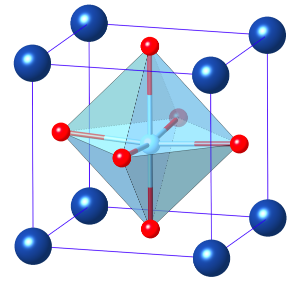
\includegraphics[width=0.75\textwidth]{figures/material}
	    \end{figure}
	\end{column}
    \end{columns}
    \bigskip
  \color{ForestGreen}
  We envision constructing a new generation of pseudopotentials that are highly accurate and isospectral to the original many-body Hamiltonian:
  \begin{itemize}
    \item<2->[$\rightarrow$] \color{ForestGreen}{\underline{Many-body construction}.} \color{black}{Constructed from relativistic {\it many-body} spectra leading to the reproduction of {\it nearly exact} many-body properties.}
    \item<3->[$\rightarrow$] \color{ForestGreen}{\underline{Reliable and universal}.} \color{black}{Tested and validated in many-body framework. Usable in both mean-field and many-body methods (in the spirit of the original all-electron $H$)}
 %   \item<4>[$\rightarrow$] \color{ForestGreen}{\underline{Simple and compact}.} \color{black}{As a first attempt, we try to use a form that is as simple as possible and find its accuracy limits}
  \end{itemize}
    
\end{frame}

\subsection{ECP Parametrization}
\begin{frame}
    \begin{block}
	{ECP Parametrization}
	We choose a semi-local parametrization for the ECPs.\\ 
    \end{block}
    \begin{center}
        \begin{tcolorbox}[enhanced,drop lifted shadow,boxrule=0.1pt,colback=blue!15,width=0.41\textwidth]
            $H_{\rm val} = \sum\limits_i \left[ T_i^{\rm kin}+ V_i^{\rm pp} \right] +  \sum\limits_{i<j}\frac{1}{r_{ij}}$
        \end{tcolorbox}
    \end{center}
    where 
    \begin{equation*}
	V_i^{\rm pp} = V_{\rm loc}(r_i) + \sum\limits_{\ell = 0} V_{\ell}(r_i) | \ell m \rangle \langle \ell m |, \quad V_\ell(r) = \sum_{k=1} \beta_{\ell k} e^{-\alpha_{\ell k}r^2}
    \end{equation*}
    and the local channel is finite at the origin
    \begin{equation*}
	V_{\rm loc}(r) = -\frac{Z_{\rm eff}}{r}\left( 1-e^{-\alpha r^2} \right) + \alpha Z_{\rm eff} r e^{-\beta r^2} + \sum_{k=1} \gamma_k e^{-\delta_i r^2}
    \end{equation*}
\end{frame}

\subsection{ECP Construction}
\begin{frame}
    {\color{ForestGreen}Many-body spectra and norm-conservation}
    \begin{itemize}
        \item Total Objective Function: \\
            $ \mathcal{O}^2 = \omega_0 \mathcal{E}^2 + \omega_1 \mathcal{N}^2 $, where $\omega_0,\omega_1$ are tunable weights\\
        \item CCSD(T) energy consistency:\\
            $\mathcal{E}^2 = \sum_s \left( \Delta E_s^{\rm ECP } -\Delta E_s^{\rm AE} \right)^2$, note that $\Delta E_s^{\rm AE}$ agrees with experiment to $\le 0.03$~eV
        \item Norm-conservation: \\
        $\mathcal{N}^2 = \sum_\ell\left( N_\ell^{\rm ECP}-N_\ell^{\rm AE} \right)^2 + \left(V_\ell^{\rm ECP} - V_\ell^{\rm AE}\right)^2 + \left(S_\ell^{\rm ECP}-S_\ell^{\rm AE}\right)^2 + \left( \epsilon_\ell^{\rm ECP} - \epsilon_\ell^{\rm AE} \right)^2$ where \\
        $N_\ell$: norm inside cutoff radius, $V_\ell, S_\ell, \epsilon_\ell$: value, derivative, eigenvalue of the orbital
    \end{itemize}
\end{frame}

\subsection{Main Group Elements}
\begin{frame}

  \large

  {\color{NavyBlue}Discrepancies from AE atomic spectrum \& CCSD(T) binding curve: }%{\color{RedOrange}\quad$\sum_s\big(\Delta E_s^{ECP}-\Delta E_s^{AE}\big)^2$}}

%  \bigskip
%  {\color{ForestGreen} CCSD(T) and Spectral  optimization: } \only<2>{{\color{red} (with FC)}}

  \only<1-1>{
  \begin{columns}
    \begin{column}{0.5\textwidth}
    \vfill
    \centering
    {\Large \color{blue}{O Atomic Spectrum (eV)} }
    \bigskip
     
    \small
    \begin{tabular}{lrrc}
     \hline
     \hline
     Core Approx. & $\Delta$IP(I) & $\Delta$EA & MAD \\
     \hline
     UC          & $ -0.0142 $ & $ -0.0017 $ & $ 0.0865 $ \\  
     BFD         & $ -0.0438 $ & $ -0.0105 $ & $ 0.3275 $ \\ 
     TN-DF       & $ -0.0436 $ & $ -0.0092 $ & $ 0.2669 $ \\
     TN-CEPP     & $ -0.0192 $ & $ -0.0259 $ & $ 0.1442 $ \\
     TN-eCEPP    & $ -0.0053 $ & $  0.0083 $ & $ 0.1434 $ \\
     \hline
     Spectral    & $ -0.0058 $ & $ -0.0044 $ & $ 0.0078 $ \\
     Spatial     & $ -0.0118 $ & $  0.0012 $ & $ 0.1303 $ \\
     Spec/Space  & $  0.0083 $ & $  0.0036 $ & $ 0.0192 $ \\
     \hline
     \hline
    \end{tabular}
    \end{column}
    \begin{column}{0.5\textwidth}
      \begin{figure}
        \centering
        \vspace*{-0.05\textheight}
        \begin{tikzpicture}
          \node[inner sep=0] at (0,0) {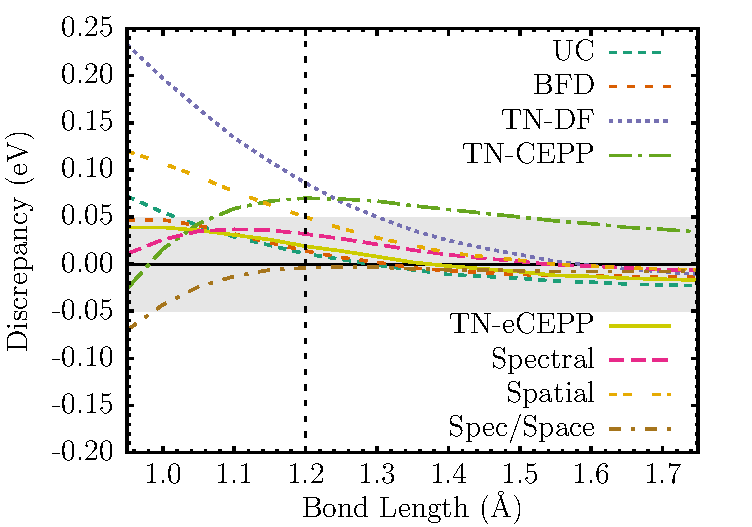
\includegraphics[width=\textwidth]{figures/o2_all_diffs}};
          \node at (0,3.0) {\Large \color{blue}{O$_2(^3\Sigma_g)$} };
          \draw[red, thick, ->] (-2.65,-2.65) node[anchor=north] {\tiny Near Dissociation Threshold} (-2.5,-2.75)  -- (-2.5,-2.3);
          \draw[red, thick, ->] (0,2) node[anchor=west] (0.6,0) {\tiny All-electron $R_0$} -- (-0.5,2);
        \end{tikzpicture}
      \end{figure}
    \end{column}
  \end{columns}
  }
  \only<2-2>{
  \begin{columns}
    \begin{column}{0.5\textwidth}
    \vfill
    \centering
    {\Large \color{blue}{O Atomic Spectrum (eV)} }
    \bigskip
     
    \small
    \begin{tabular}{lrrc}
     \hline
     \hline
     Core Approx. & $\Delta$IP(I) & $\Delta$EA & MAD \\
     \hline
     UC          & $ -0.0142 $ & $ -0.0017 $ & $ 0.0865 $ \\  
     BFD         & $ -0.0438 $ & $ -0.0105 $ & $ 0.3275 $ \\ 
     TN-DF       & $ -0.0436 $ & $ -0.0092 $ & $ 0.2669 $ \\
     TN-CEPP     & $ -0.0192 $ & $ -0.0259 $ & $ 0.1442 $ \\
     TN-eCEPP    & $ -0.0053 $ & $  0.0083 $ & $ 0.1434 $ \\
     \hline
     \color{darkblue} Spectral    & \color{darkblue}$ -0.0058 $ & \color{darkblue}$ -0.0044 $ & \color{darkblue}$ 0.0078 $ \\
     Spatial     & $ -0.0118 $ & $  0.0012 $ & $ 0.1303 $ \\
     Spec/Space  & $  0.0083 $ & $  0.0036 $ & $ 0.0192 $ \\
     \hline
     \hline
    \end{tabular}
    \end{column}
    \begin{column}{0.5\textwidth}
      \begin{figure}
        \centering
        \vspace*{-0.05\textheight}
        \begin{tikzpicture}
          \node[inner sep=0] at (0,0) {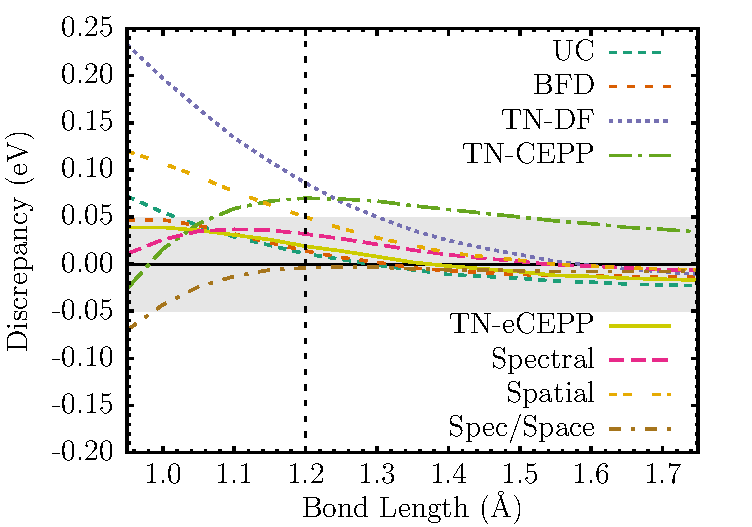
\includegraphics[width=\textwidth]{figures/o2_all_diffs}};
          \node at (0,3.0) {\Large \color{blue}{O$_2(^3\Sigma_g)$} };
          \draw[red, thick, ->] (-2.65,-2.65) node[anchor=north] {\tiny Near Dissociation Threshold} (-2.5,-2.75)  -- (-2.5,-2.3);
          \draw[red, thick, ->] (0,2) node[anchor=west] (0.6,0) {\tiny All-electron $R_0$} -- (-0.5,2);
        \end{tikzpicture}
      \end{figure}
    \end{column}
  \end{columns}
  }
\end{frame}

\begin{frame}

  \large

  \onslide<1->{\color{NavyBlue}Transferability Testing}
\begin{figure}
  \color{black}
  \centering
  \subfloat{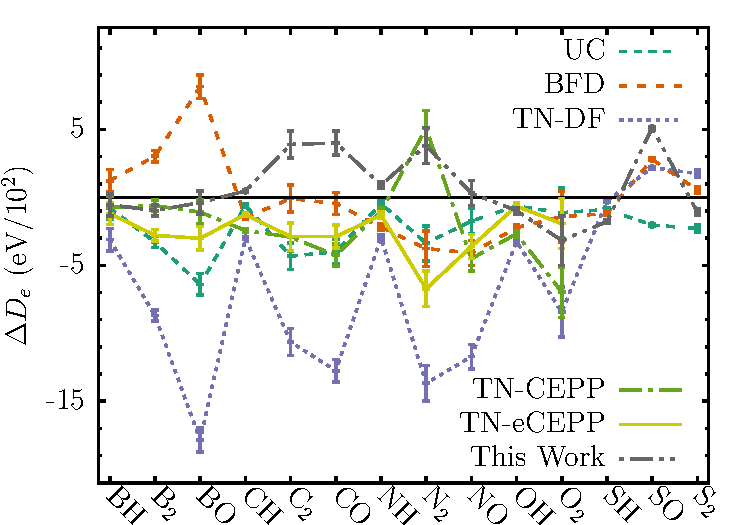
\includegraphics[height=0.45\textheight,width=0.33\textwidth]{figures/de.pdf}}
  \subfloat{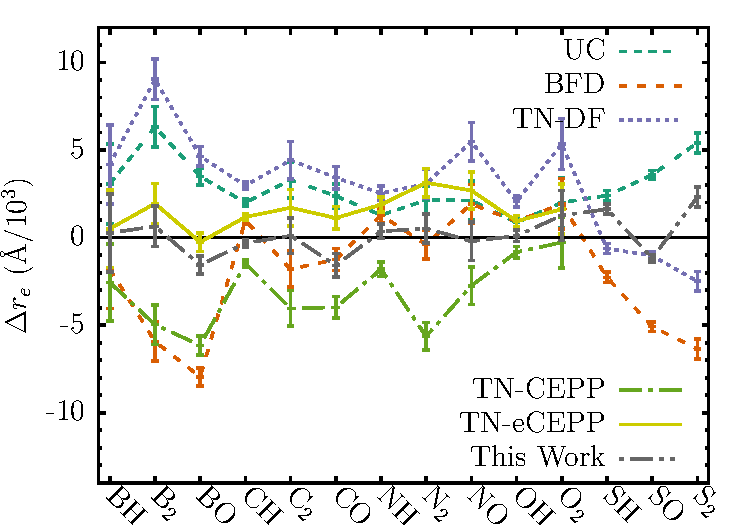
\includegraphics[height=0.45\textheight,width=0.33\textwidth]{figures/re.pdf}}
  \subfloat{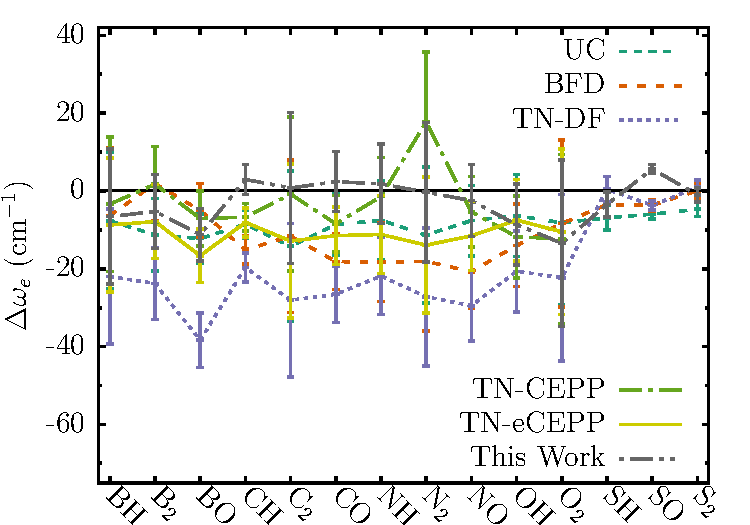
\includegraphics[height=0.45\textheight,width=0.33\textwidth]{figures/we.pdf}}
\end{figure}

\small
\centering
\color{black}
    \begin{tabular}{c | cccccc}
	\hline
	\hline
	       MAD   &   UC  &   BFD  &    TN-DF &   TN-CEPP &  TN-eCEPP &   This Work \\
	\hline
	 $D_e$    (  eV/$10^2$)     &    {\color{ForestGreen}\bf 2.0(2)} &     6.9(2) &     2.3(2) &     2.9(3) &     2.6(3) &   {\color{ForestGreen}\bf 2.0(2)}   \\
	 $r_e$      (\AA/$10^3$)    &    2.9(3) &     2.8(3) &     3.7(3) &     3.1(3) &     1.5(3) &   {\color{ForestGreen}\bf 0.9(3)}   \\
	 $\omega_e$ (cm$^{-1}$)     &      9(3) &      10(3) &      20(3) &       7(4) &      11(4) &     {\color{ForestGreen}\bf 5(3)}   \\
	 $D_{diss}$      (eV/$10^2$)      &    13.10 &      19.96 &     11.75  &     20.94   &     7.79 &       {\color{ForestGreen}\bf 5.75} \\
	 \hline
	 \hline
    \end{tabular}

\end{frame}

\subsection{Transition Metals}
\begin{frame}
    \begin{columns}
	\begin{column}
	    {0.5\textwidth}
	    \begin{itemize}
		\footnotesize
	        \item[] {\bf AE Reference:} RCCSD(T) correlating {\em all} electrons\\
		\item[] {\color[HTML]{E41A1C} \bf UC:} is a uncorrelated Ne-core RCCSD(T)  \\
		\item[] {\color[HTML]{377EB8} \bf BFD:} Burkatzki-Filippi-Dolg DHF ECPs for QMC\\
		        {\color[HTML]{4DAF4A} \bf  STU:} Stuttgart group DHF ECPs\\
			{\color[HTML]{984EA3} \bf TN17:} Trail-Needs correlated ECPs for QMC \\
			{\color[HTML]{FF7F00} \bf Our ccECP:} Our correlation-consistent ECP
		\item[]
		\item[] {\color{wolfred} \bf Discrepancy:} \\
		    \begin{tcolorbox}[enhanced,drop lifted shadow,boxrule=.1pt,colback=blue!15,width=0.75\textwidth]
			    \centering
	        	    $\left(E_{s}^{\rm ECP}-E_{\rm GS}^{\rm ECP}\right) - \left( E_{s}^{\rm AE} - E_{\rm GS}^{\rm AE} \right) $
	        	\end{tcolorbox}
	    \end{itemize}
	\end{column}
	\begin{column}
	    {0.55\textwidth}
	    \only<1-1>{
   	   	 \begin{figure}[h]
   	   	     \centering
	   	     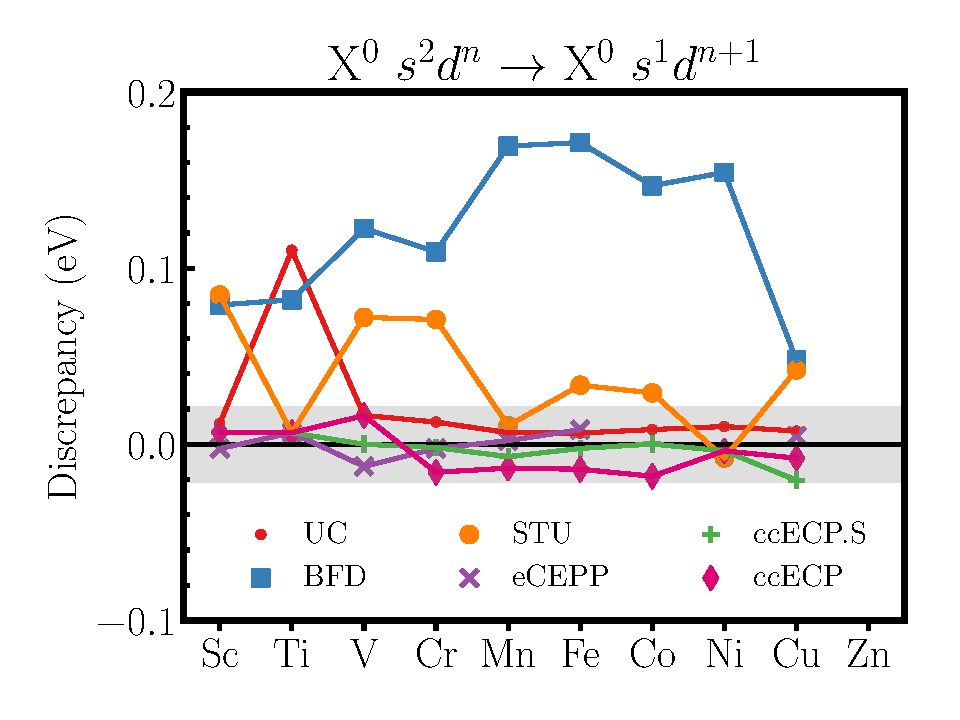
\includegraphics[width=\textwidth]{figures/Is2dn_to_Is1dn1}
   	   	 \end{figure}
	    }
	    %\only<2-2>{
   	    %    \begin{figure}[h]
   	    %        \centering
	    %        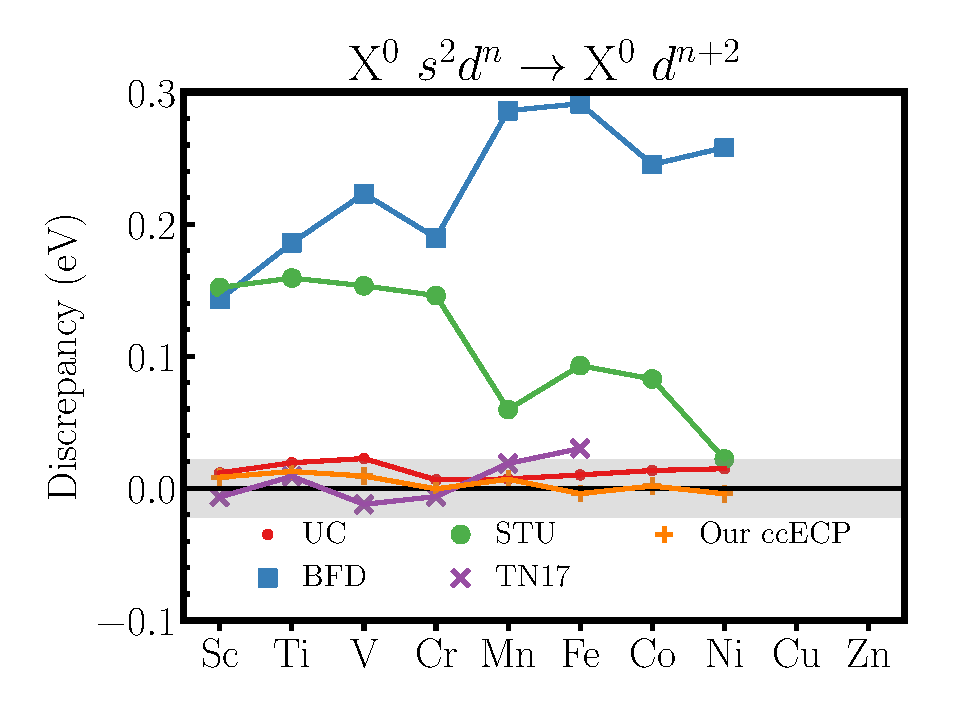
\includegraphics[width=\textwidth]{figures/Is2dn_to_Idn2}
   	    %    \end{figure}
	    %}
	    %\only<3-3>{
   	    %    \begin{figure}[h]
   	    %        \centering
	    %        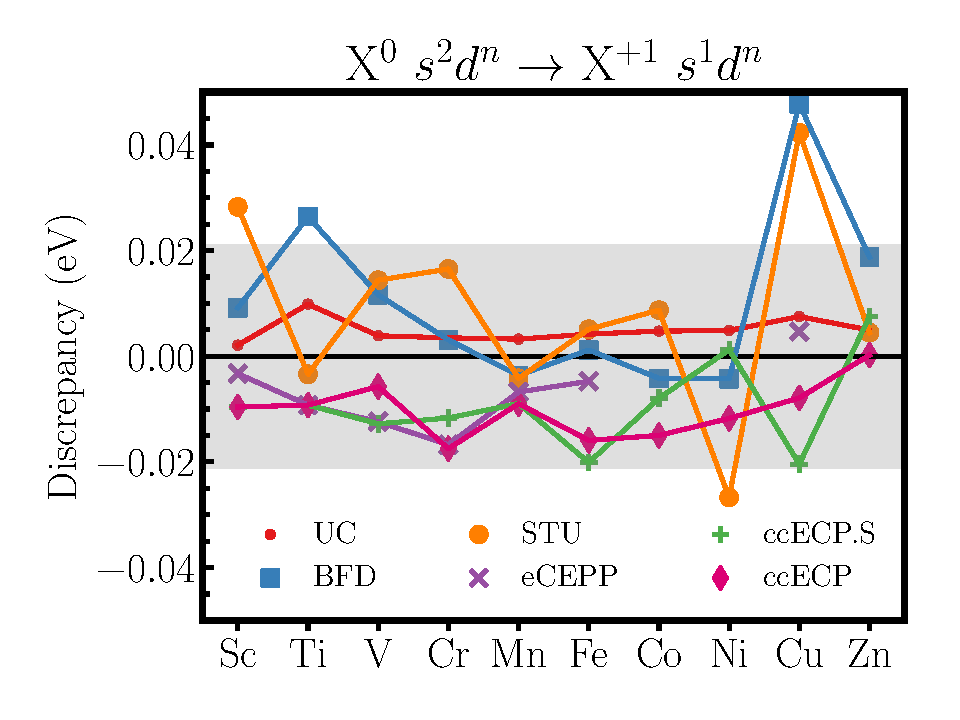
\includegraphics[width=\textwidth]{figures/Is2dn_to_IIs1dn}
   	    %    \end{figure}
	    %}
	    %\only<4-4>{
   	    %    \begin{figure}[h]
   	    %        \centering
	    %        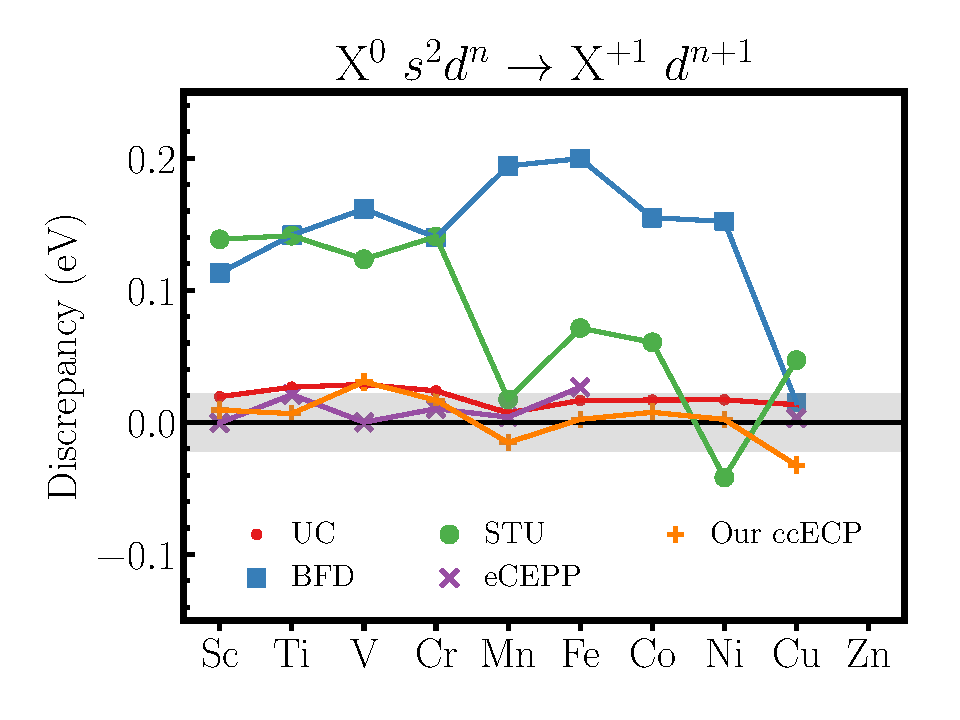
\includegraphics[width=\textwidth]{figures/Is2dn_to_IIdn1}
   	    %    \end{figure}
	    %}
	    %\only<5-5>{
   	    %    \begin{figure}[h]
   	    %        \centering
	    %        \includegraphics[width=\textwidth]{figures/ea}
   	    %    \end{figure}
	    %}
	    \only<2-2>{
   	        \begin{figure}[h]
   	            \centering
	            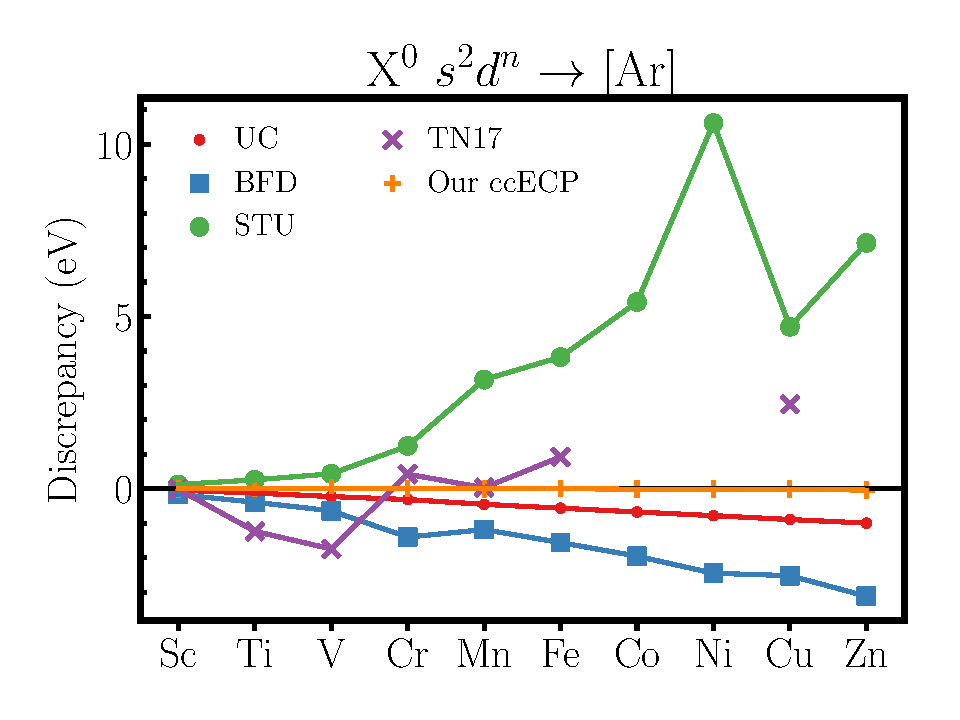
\includegraphics[width=\textwidth]{figures/ar}
   	        \end{figure}
	    }
	\end{column}
    \end{columns}
\end{frame}

\begin{frame}
    \begin{columns}
	\begin{column}
	    {0.45\textwidth}
	    \begin{block}
		{Example Spectrum (Ni)}
                \begin{table}
		    \scriptsize
                \centering
                \begin{tabular}{ll|ll}
		{[Ar] $3d^84s^2$ }  & $^3F$ &  {[Ar] $3d^5$ }      & $^6S$\\
                {[Ar] $3d^94s^1$ }  & $^3D$ &  {[Ar] $3d^4$ }      & $^5D$\\ 
                {[Ar] $3d^{10}$ }   & $^1S$ &  {[Ar] $3d^3$ }      & $^4F$\\
                {[Ar] $3d^84s^1$ }  & $^4F$ &  {[Ar] $3d^2$ }      & $^3F$\\
                {[Ar] $3d^9$ }      & $^2D$ &  {[Ar] $3d^1$ }      & $^2D$\\
                {[Ar] $3d^8$ }      & $^3F$ &  {[Ar] }             & $^1S$\\
                {[Ar] $3d^7$ }      & $^4F$ &  {[Ne] $3s^2$ }      & $^1S$\\
                {[Ar] $3d^6$ }      & $^5D$ &  {[Ar] $3d^94s^2$ }  & $^2D$\\
                \end{tabular}
                \end{table}
	    \end{block}
	    {\color{wolfred}Mean Absolute Deviation:}
	    \small{
		\begin{tcolorbox}[enhanced,drop lifted shadow,boxrule=0.1pt,colback=blue!15]
		    $\frac{1}{N}\sum\limits_{s=1}^N \left| \left( E_s^{\rm PP}-E_{\rm GS}^{\rm PP} \right) - \left( E_s^{\rm AE}-E_{GS}^{\rm AE} \right)\right| $
	        \end{tcolorbox}
	    }
	\end{column}
	\begin{column}
	    {0.55\textwidth}
   	     \begin{figure}[h]
   	         \centering
		 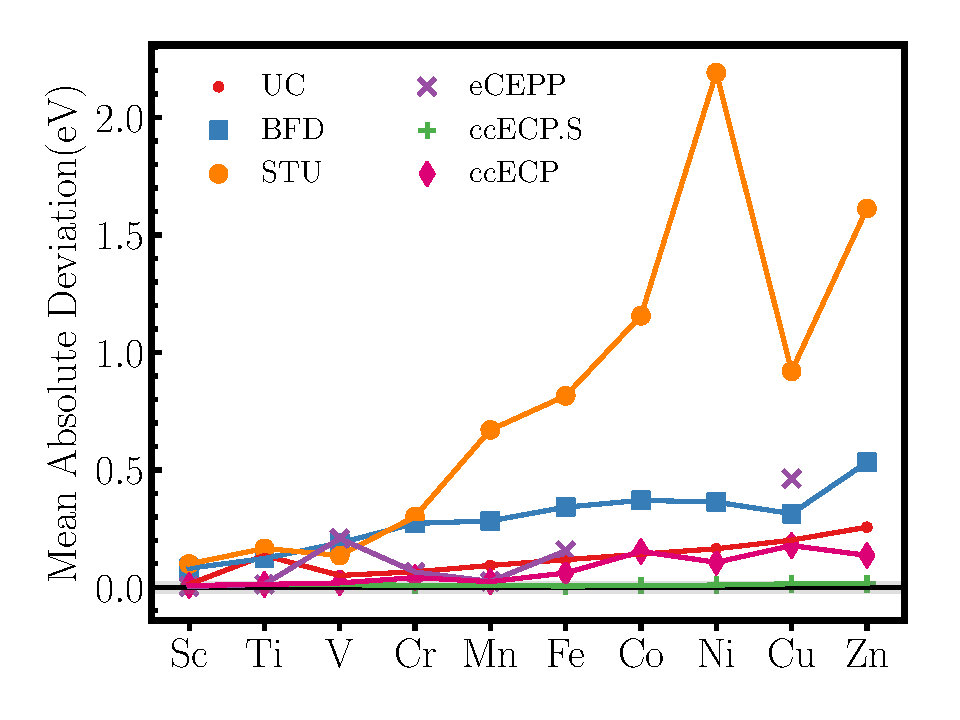
\includegraphics[width=\textwidth]{figures/mad}
   	     \end{figure}
	\end{column}
    \end{columns}
\end{frame}

\subsection{Transferability with Selected Molecules}

\begin{frame}
    \begin{center}
	{\Large\color{wolfred}{\bf Monoxides}}
    \end{center}
    \begin{columns}
	\begin{column}
	    {0.5\textwidth}
	    \begin{figure}[h]
		\centering
		\caption*{ScO binding curve discrepancies}
		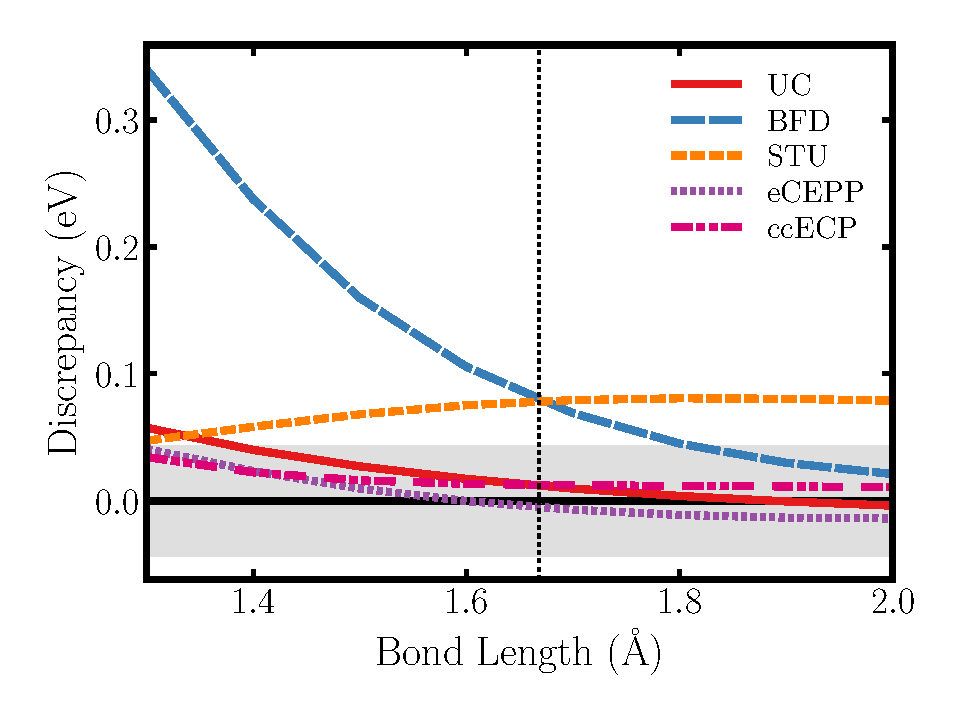
\includegraphics[width=\textwidth]{figures/ScO}
	    \end{figure}
	\end{column}
	\begin{column}
	    {0.5\textwidth}
	    \begin{figure}[h]
		\centering
		\caption*{VO binding curve discrepancies}
		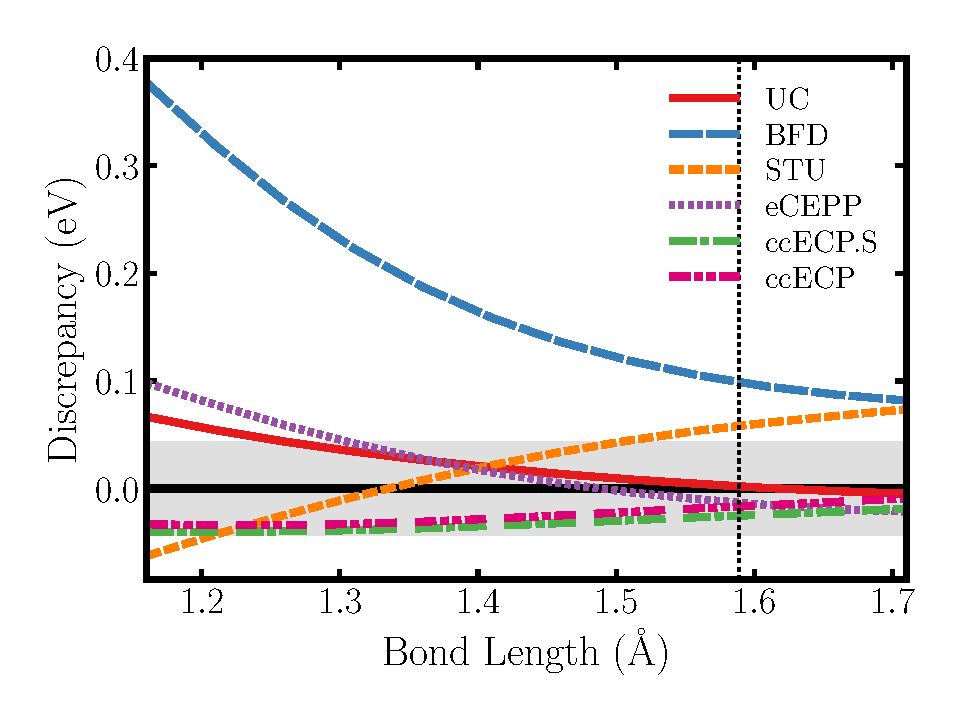
\includegraphics[width=\textwidth]{figures/VO}
	    \end{figure}
	\end{column}
    \end{columns}
\end{frame}


\section{Quantum Chemistry Examples}
\subsection{Website}
\begin{frame}
    \begin{columns}
	\begin{column}
	    {0.4\textwidth}
	    {\color{darkblue} http://pseudopotentiallibrary.org}
	    \scriptsize
	    \begin{itemize}
		\item[] Updated as new correlated ECPs are developed
		\item[]
		\item[] Anyone can contribute ECPs through \url{http://github.com/QMCPACK/pseudopotentiallibrary}
		\item[]
		\item[] Soon will include completed table up through Kr
		\item[]
        \item[] KB projectors for {\it some} atoms are available, will update as they become available
	    \end{itemize}
	\end{column}
	\begin{column}
	    {0.6\textwidth}
	    \begin{figure}[h]
		\centering
		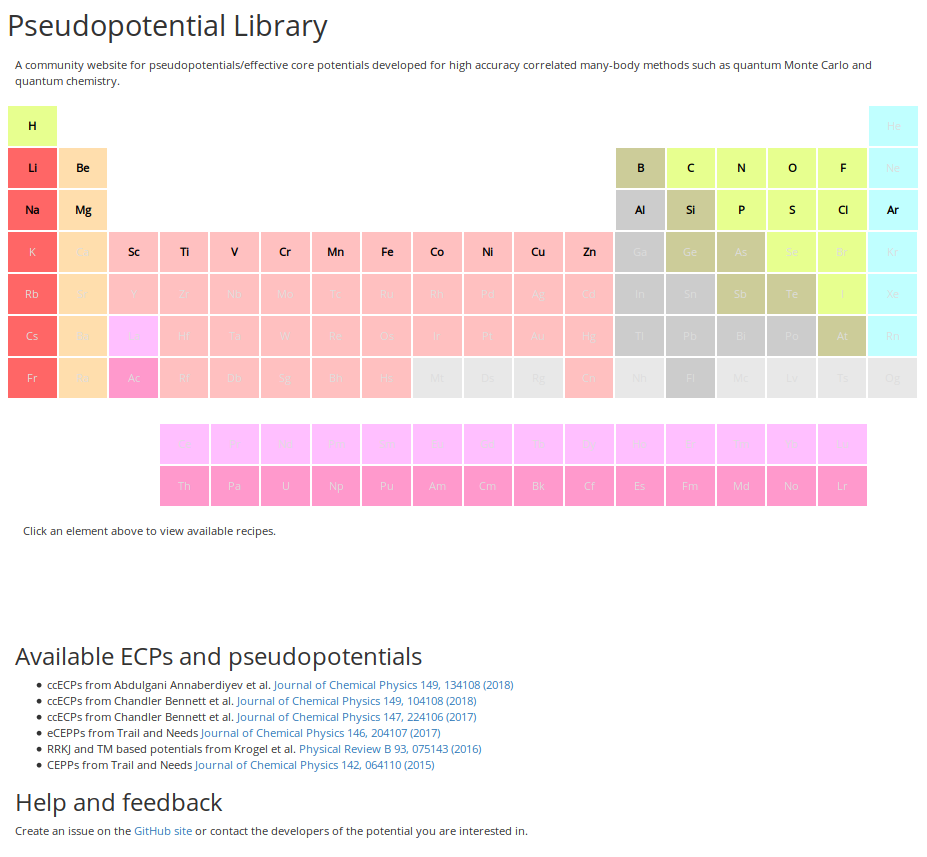
\includegraphics[width=0.8\textwidth]{figures/pseudopotentiallibrary}
	    \end{figure}
	\end{column}
    \end{columns}
\end{frame}

\begin{frame}
    \begin{columns}
	\begin{column}
	    {0.3\textwidth}
        {\color{wolfred} ccECP format} 
        \tiny
            \hfil $V_\ell(r) = \sum\limits_{k=1}^{N_\ell} \beta_k r^{n_k-2} e^{-\alpha_k r^2}$
        \begin{eqnarray*}
            \begin{array}{ccc}
                Z_{\rm eff} & L+1 \\
                N_0 & \ldots & N_{L} 
            \end{array}\\
            \left.
            \begin{array}{ccc}
                n_1 & \alpha_1 & \beta_1 \\
                \vdots & \vdots & \vdots \\
                n_{N_0} & \alpha_{N_0} & \beta_{N_0}
            \end{array}\right\} \ell=0 \\
            \begin{array}{ccc}
                & \vdots 
            \end{array}\\
            \left.
            \begin{array}{ccc}
                    n_1 & \alpha_1 & \beta_1 \\
                    \vdots & \vdots & \vdots \\
                    n_{N_L} & \alpha_{N_L} & \beta_{N_L}
            \end{array}\right\} \ell=L
        \end{eqnarray*}
        {\normalsize \color{darkblue} Carbon Example}
        \lstinputlisting{C.ccECP}
	\end{column}
	\begin{column}
	    {0.7\textwidth}
	    %\begin{figure}[h]
		%\centering
		%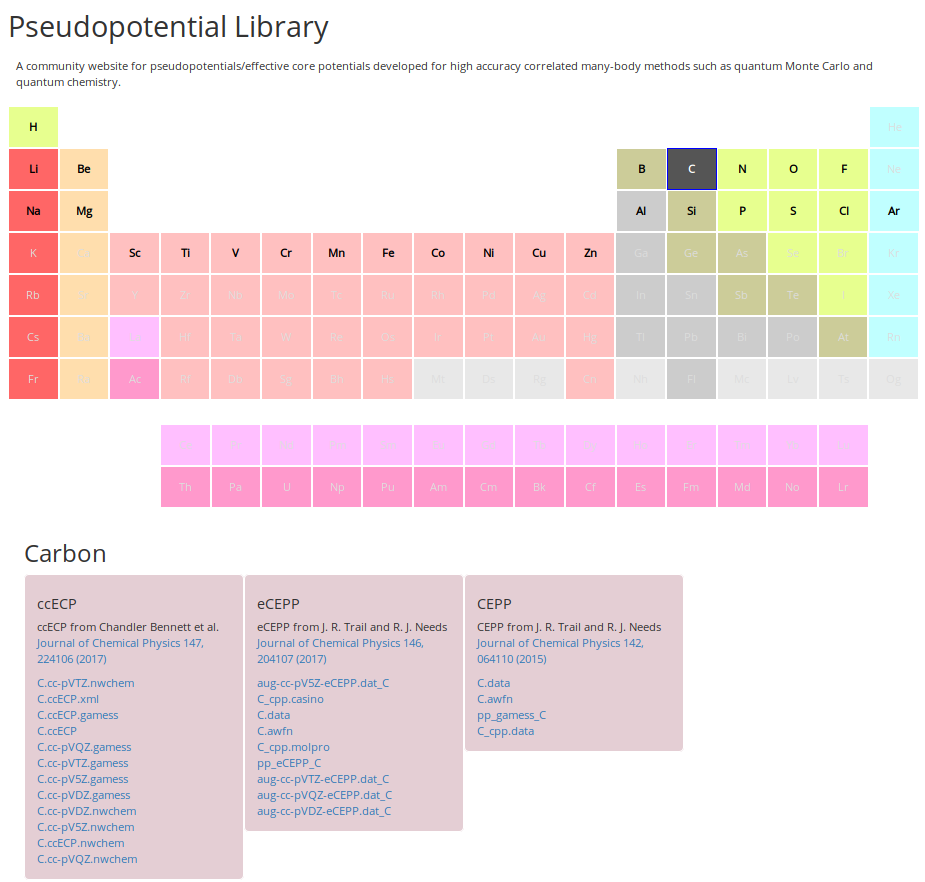
\includegraphics[width=0.8\textwidth]{figures/carbon-web}
	    %\end{figure}
		\begin{tikzpicture}
            \node [anchor=west] (water) at (-1,1.2) {\footnotesize C.ccECP};
		\begin{scope}[xshift=1.5cm]
		    \node[anchor=south west,inner sep=0] (image) at (0,0) {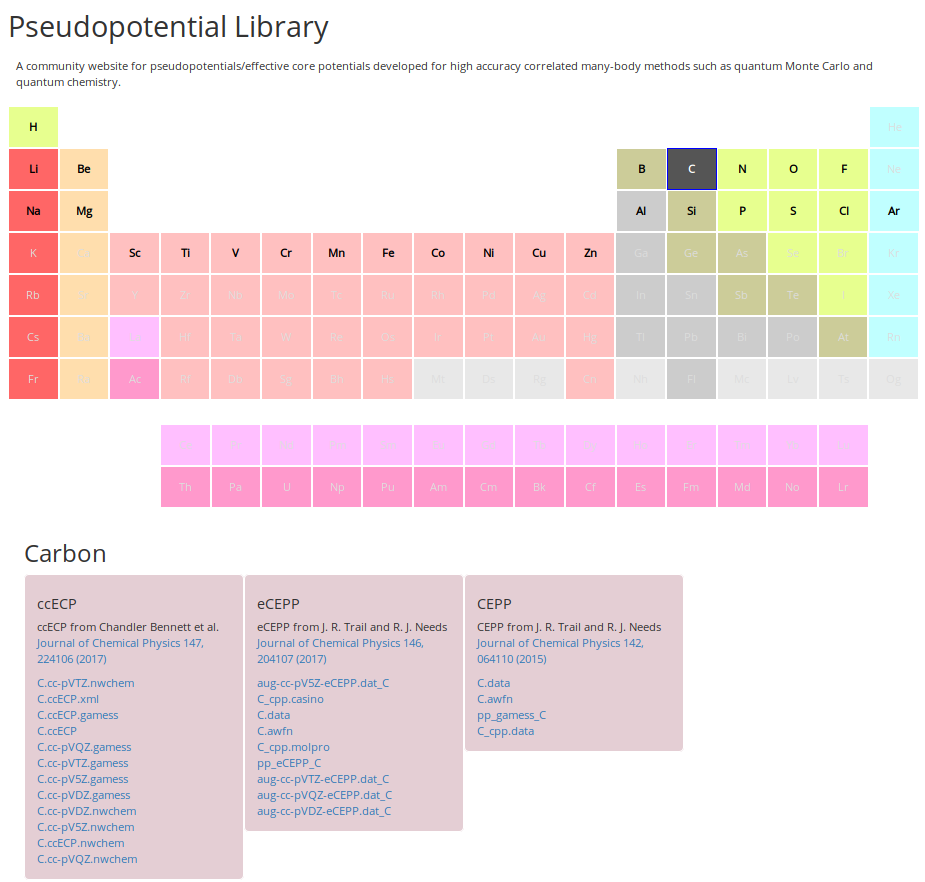
\includegraphics[width=0.7\textwidth]{figures/carbon-web}};
		    \begin{scope}[x={(image.south east)},y={(image.north west)}]
		        \draw [-stealth, line width=1pt, wolfred] (water) -- ++(0.24,0.0);
		    \end{scope}
		\end{scope}
		\end{tikzpicture}%
	\end{column}
    \end{columns}
\end{frame}

\begin{frame}
    {Available Quantum Chemistry Formats}
    For each ccECP, we include a variety of basis sets and pseudopotential formats for various codes, including cc-pV$n$Z and aug-cc-pV$n$Z basis sets, with $n \in \{\rm D,T,Q,5\}$.\\
    \bigskip
    Basis/ECP formats included for each code QMCPACK interfaces to
    \begin{enumerate}
        \item[] \textsc{\color{ForestGreen}GAMESS}: Basis sets and pseudopotential format\\
            {\hfil e.g. {\color{NavyBlue} C.cc-pVTZ.gamess \& C.ccECP.gamess}}
        \item[] \textsc{\color{Plum}Quantum Package}: Uses \textsc{GAMESS} file formats\\
            {\hfil e.g. {\color{NavyBlue} C.cc-pVTZ.gamess \& C.ccECP.gamess}}
        \item[] \textsc{\color{RedOrange}PySCF}: Parses \textsc{NWChem} formats\\
            {\hfil e.g. {\color{NavyBlue} C.cc-pVTZ.nwchem \& C.ccECP.nwchem}}
        \item[] \textsc{\color{wolfred}Qmcpack}: Uses qmcpack xml format\\
            {\hfil e.g. {\color{NavyBlue} C.ccECP.xml}}
    \end{enumerate}
\end{frame}

\subsection{Example}
\begin{frame}
    {PySCF Example: Catom.py}
    \small
    \lstset{language=Python,basicstyle=\ttfamily,keywordstyle=\color{blue}\ttfamily,commentstyle=\color{ForestGreen}\ttfamily,stringstyle=\color{red}\ttfamily,showstringspaces=false}
    \only<1-1>{\lstinputlisting[firstline=1,lastline=9]  {../files/quantum_chemistry/Catom.py}}
    \only<2-2>{\lstinputlisting[firstline=11,lastline=24]{../files/quantum_chemistry/Catom.py}}
    \only<3-3>{\lstinputlisting[firstline=26,lastline=37]{../files/quantum_chemistry/Catom.py}}
    \only<4-4>{\lstinputlisting[firstline=38,lastline=48]{../files/quantum_chemistry/Catom.py}}
\end{frame}


\section{Solid State Examples}
\begin{frame}
    {Using ccECPs for solid state}
    \begin{itemize}
        \item If using gaussian basis sets, i.e. (PySCF), our potentials can be used as is, as shown previously.
        \item Using PBC, basis sets may need to be altered and/or reoptimized entirely. e.g. Diffuse functions can cause linear dependency issues, to fix add: \\
            {\color{darkblue}cell.drop\_exponent=0.1} in pySCF to the cell object
        \item If basis is problematic, contractions for occupied orbitals need to be tailored to the ECP. Often useful to use an ionized +1, +2 state to get contractions.\\
            Uncontracted primitives can come from existing solid-state basis sets. \\
            For inspiration, can use primitives from \url{http://www.crystal.unito.it/basis-sets.php} or \\
            \url{https://www.tcm.phy.cam.ac.uk/~mdt26/crystal.html}
    \end{itemize}
\end{frame}

\subsection{KB Transformation}
\begin{frame}
    \begin{columns}
        \begin{column}
            {0.4\textwidth}
            \centering
            {\color{ForestGreen}Semi-local potential}\\
            $\hat{V}_{\rm SL} = \sum\limits_{\ell m}  | \ell m\rangle V_\ell(r) \langle\ell m|$
        \end{column}
        \begin{column}
            {0.6\textwidth}
            \centering
            {\color{ForestGreen}KB potential}\\
            $\hat{V}_{\rm KB} = V_{\rm local}(r) + \sum\limits_{\ell m} \frac{| \phi_{\ell m}^{\rm PS} \delta V_\ell \rangle \langle \delta V_\ell \phi_{\ell m}^{\rm PS}|}{\langle \phi_{\ell m}^{\rm PS} |\delta V_\ell | \phi_{\ell m}^{\rm PS}\rangle} $
        \end{column}
    \end{columns}
    \bigskip
    \begin{itemize}
        \item[] {\color{NavyBlue} Ghost States:} Low energy states that have the wrong number of nodes. Can cause unphysical energies, difficulty, optimizing wave functions, unstable DMC, etc. (see Drummond, Trail, \& Needs, PRB {\bf 94}, 165170 (2016)).
        \item[] {\color{NavyBlue} Transferability:} Ability of a potential to perform the same as the reference. 
    \end{itemize}
    \bigskip

    We take our semi-local ccECPs to be an accurate representation of the AE Hamiltonian. Therefore, we need the KB version to be transferable with respect to the semi-local potential.

\end{frame}

\begin{frame}
    OPIUM is a norm-conserving pseudopotential generation tool to develop pseudopotentials for plane-wave codes like QE.\\
    \bigskip
    A modified version that can input gaussian parameterized semi-local potentials (ccECPs, Stuttgart, BFD, etc) has been used to generate the UPF files, and included some information about ghost states, transferability, recommended plane-wave cutoffs, in the .rpt file.
\end{frame}

\begin{frame}
    \begin{columns}
        \begin{column}
            {0.3\textwidth}
		    \begin{tikzpicture}
                \node [anchor=west] (water) at (0.25,0.35) {};
		        \begin{scope}[xshift=1.5cm]
		            \node[anchor=south west,inner sep=0] (image) at (0,0) {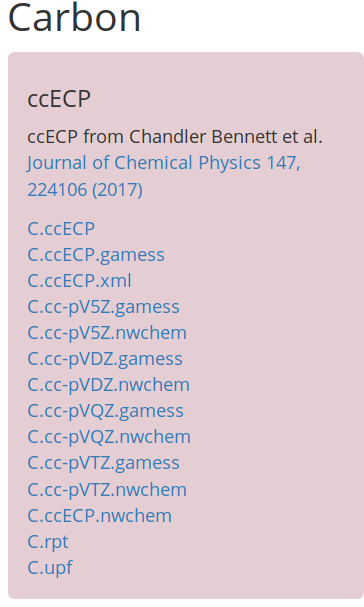
\includegraphics[width=0.5\textwidth]{figures/carbon_snapshot}};
		            \begin{scope}[x={(image.south east)},y={(image.north west)}]
                        \draw [-stealth, line width=1pt, wolfred] (water) -- ++(0.5,-0.025);
                        \draw [-stealth, line width=1pt, wolfred] (water) -- ++(0.5,0.025);
		            \end{scope}
		        \end{scope}
		    \end{tikzpicture}%
        \end{column}
        \begin{column}
            {0.7\textwidth}
            \centering
            \tiny
            \only<1-1>{
                {\color{ForestGreen} \small Ghost States}
                \lstinputlisting[firstline=82,lastline=100]{C.rpt}
            }
            \only<2-2>{
                {\color{ForestGreen} \small Suggested Cutoff}
                \lstinputlisting[firstline=104,lastline=125]{C.rpt}
            }
            \only<3-3>{
                {\color{ForestGreen} \small Transferability}
                \lstinputlisting[firstline=127,lastline=143]{C.rpt}
            }
        \end{column}
    \end{columns}
    \bigskip
    \only<1-1>{
        \color{NavyBlue}Information about existence of ghosts for the semi-local and non-local evaluation
    }
    \only<2-2>{
        \color{NavyBlue}Suggested cutoffs for the projectors. Here, $\sim240$~Ry. Choose max from each atom!
    }
    \only<3-3>{
        \color{NavyBlue}Transferability of projector wrt semi-local potential. Small errors, especially for low lying states
    }
\end{frame}


\section{Conclusions}
\begin{frame}
    \begin{itemize}
        \item Each ccECP that has been developed has a {\it .nwchem \& .gamess} extension, which allows them to be used with \textsc{GAMESS}, \textsc{PySCF}, and  \textsc{Quantum Package} using the appropriate format. 
        \item The number of UPF files is currently limited, but will be updated as they are generated and tested. For transition metals, a good alternative is to use the projectors from Jaron Krogel, listed under RRKJ\_PRB\_93\_075143 and TM\_PRB\_93\_075143. 
        \item To proceed further, simply download the XML potential for \textsc{QMCPACK} and run the appropriate converter to generate the files (convert4qmc for  \textsc{Quantum Package}, \textsc{PySCF}, and \textsc{GAMESS} and pw2qmcpack for \textsc{Quantum Espresso} and proceed with your QMC workflow.
    \end{itemize}
\end{frame}

\end{document}
